\newcommand\vect[1]{{\left(\begin{array}{c}#1\end{array}\right)}}

\begin{aufgabe}
	Bestimmen Sie den Schwerpunkt der folgenden Körper.

	\begin{center}
		\Spalten{0.49}{
	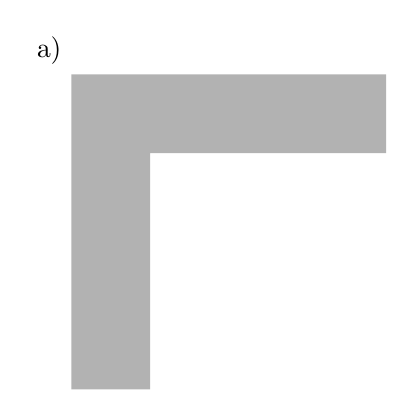
\begin{tikzpicture}
	\def\DX{4}%in x richtung
	\def\DY{4}%in y richtung
	\def\DB{1}%breite
	\draw (0,0) node [above left] {a)};
	\fill [color=black!30] (0,0)--++(\DX,0)--++(0,-\DB)--++(-\DX+\DB,0)--++(0,-\DY+\DB)--++(-\DB,0)--(0,0);
	\end{tikzpicture}
}{0.49}{	
	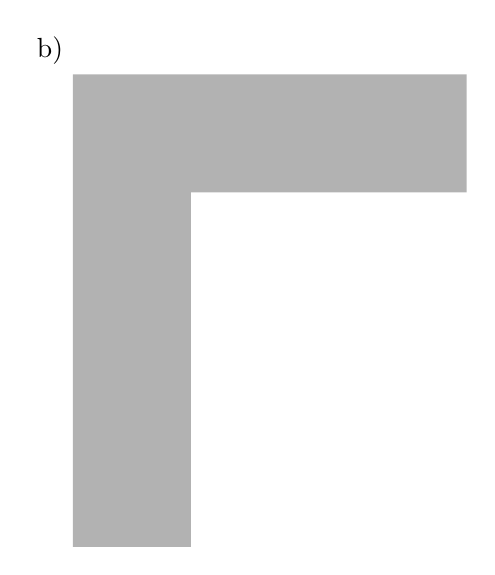
\begin{tikzpicture}
	\def\DX{5}%in x richtung
	\def\DY{6}%in y richtung
	\def\DB{1.5}%breite
	\draw (8,0) node [above left] {b)};
	\fill [color=black!30] (8,0)--++(\DX,0)--++(0,-\DB)--++(-\DX+\DB,0)--++(0,-\DY+\DB)--++(-\DB,0)--(8,0);


	\end{tikzpicture}
}
		\Spalten{0.49}{
	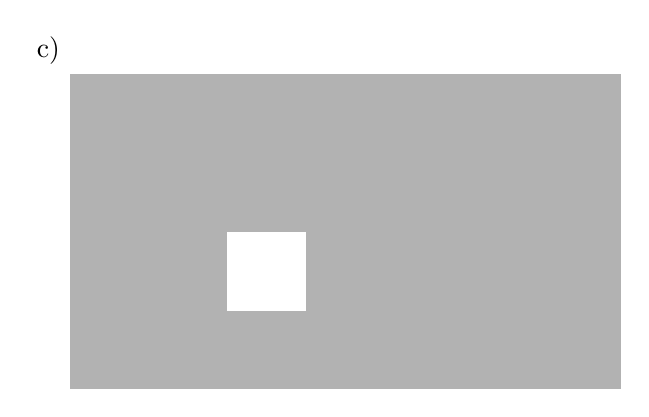
\begin{tikzpicture}
	\draw (0,0) node [above left] {c)};
	\fill [color=black!30] (0,0) rectangle (7,-4);
	\fill [color=white] (2,-2) rectangle (3,-3);
	\end{tikzpicture}
}{0.49}{	
	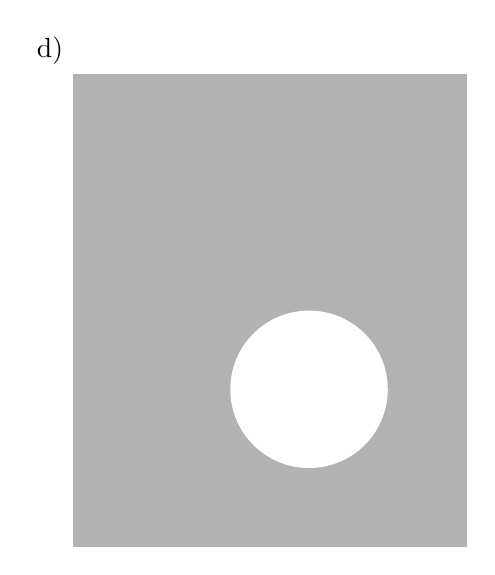
\begin{tikzpicture}
	\draw (9,0) node [above left] {d)};
	\fill [color=black!30] (9,0) rectangle (14,-6);
	\fill [color=white] (12,-4) circle (1cm);

\end{tikzpicture}
}
\end{center}

\begin{loesung}
%Loesung zu a)
	Der Schwerpunkt liegt am Schnittpunkt der zwei gepunkteten Linien.

	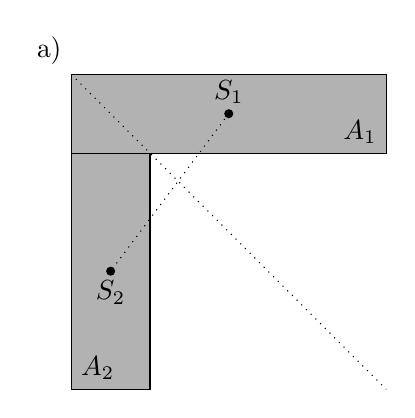
\begin{tikzpicture}
	\def\DX{4}%in x richtung
	\def\DY{4}%in y richtung
	\def\DB{1}%breite
	\draw (0,0) node [above left] {a)};
	\fill [color=black!30] (0,0)--++(\DX,0)--++(0,-\DB)--++(-\DX+\DB,0)--++(0,-\DY+\DB)--++(-\DB,0)--(0,0);
	\draw [dotted] (0,0)--(\DX,-\DY);
	
	%Umrandung der Teilflächen A1 und A2
	\draw (0,0) rectangle (4,-1) node [above left] {$A_1$};
	\draw (1,-1) rectangle (0,-4) node [above right] {$A_2$};
	%Teilschwerpunkt S1
	\coordinate (S1) at (2,-0.5);
	\draw [fill] (S1) circle (0.05) node [above] {$S_1$};
	%Teilschwerpunkt S2
	\coordinate (S2) at (0.5,-2.5);
	\draw [fill] (S2) circle (0.05) node [below] {$S_2$};

	\draw [dotted] (S1)--(S2);

	\end{tikzpicture}

	\vspace*{3cm}

%Loesung zu b)
	\Spalten{0.40}{
	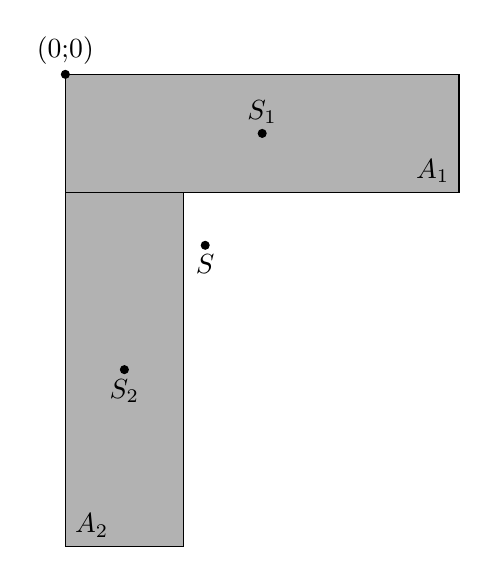
\begin{tikzpicture}
	\def\DX{5}%in x richtung
	\def\DY{6}%in y richtung
	\def\DB{1.5}%breite
%	\draw (0,0) node [above left] {b)};
	\fill [color=black!30] (0,0)--++(\DX,0)--++(0,-\DB)--++(-\DX+\DB,0)--++(0,-\DY+\DB)--++(-\DB,0)--(0,0);


	\draw [fill] (0,0) circle (0.05) node [above] {(0;0)};

	%Umrandung der Teilflächen A1 und A2
	\draw (0,0) rectangle (5,-1.5) node [above left] {$A_1$};
	\draw (1.5,-1.5) rectangle (0,-6) node [above right] {$A_2$};
	%Teilschwerpunkt S1
	\coordinate (S1) at (2.5,-0.75);
	\draw [fill] (S1) circle (0.05) node [above] {$S_1$};
	%Teilschwerpunkt S2
	\coordinate (S2) at (0.75,-3.75);
	\draw [fill] (S2) circle (0.05) node [below] {$S_2$};

	%Schwerpunkt liegt bei
	\coordinate (S) at (1.77632,-2.17105);
	\draw [fill] (S) circle (0.05) node [below] {$S$};

	\end{tikzpicture}
}{0.59}{
	Den Urspring des Koordinatensystems lege ich an die ober linke Ecke der Gesamtfläche.

	Mit dem gewählten Ursprung des Koordinatensystems liegt der Teilschwerpunkt $S_1$ bei der Koordinate $(\num{2.5};\num{-0.75})$,
	$S_2$ liegt bei $(\num{0.75};\num{-3.75})$.

	Der Schwerpunkt der Gesamtfläche liegt bei
	\begin{eqnarray*}
		\begin{split}
		r_s &=\frac{r_1\cdot A_1 + r_2\cdot A_2}{A_1 + A_2} =\\
		    &=\frac{\vect{2.5\\-0.75}\cdot\SI{7.5}{cm^2} + \vect{0.75\\-3.75}\cdot\SI{6.75}{cm^2}}{\SI{14.25}{cm^2}}=\\
            &=\frac{\vect{20.25\\-5.625} + \vect{5.0625\\-25.3125}}{\SI{14.25}{cm^2}} =
            =\frac{\vect{25.3125\\-30.9375}}{\SI{14.25}{cm^2}} =\\
            &=\vect{1.77632\\-2.17105}
		\end{split}
	\end{eqnarray*}
}
%Loesung zu c)

	\begin{tikzpicture}[scale=2]
	\draw (0,0) node [above left] {c)};
	\fill [color=black!30] (0,0) rectangle (7,-4);
	\fill [color=white] (2,-2) rectangle (3,-3);

	\fill [color=black!30] (0,0) rectangle (2,-4) node [color=black, above left] {$A_1$};
	\coordinate (S1) at (1,-2);
	\draw [fill] (S1) circle (0.05) node [above] {$S_1$};
	\fill [color=black!40] (3,0) rectangle (7,-4) node [color=black, above left] {$A_4$};
	\coordinate (S4) at (5,-2);
	\draw [fill] (S4) circle (0.05) node [above] {$S_4$};

%gemeinsamer Schwerpunkt von A1 und A4
	\coordinate (S14) at ($(S1)!0.66667!(S4)$);
	\draw [fill] (S14) circle (0.05) node [right] {$S_{14}$};

	\fill [color=black!50] (2,-2) rectangle (3,0) node [color=black, below left] {$A_2$};
	\coordinate (S2) at (2.5,-1);
	\draw [fill] (S2) circle (0.05) node [above] {$S_2$};
	\fill [color=black!60] (2,-3) rectangle (3,-4) node [color=black, above left] {$A_3$};
	\coordinate (S3) at (2.5,-3.5);
	\draw [fill] (S3) circle (0.05) node [above] {$S_3$};

%gemeinsamer Schwerpunkt von A2 und A3
	\coordinate (S23) at ($(S2)!0.33333!(S3)$);
	\draw [fill] (S23) circle (0.05) node [above] {$S_{23}$};

%Schwerpunkt
	\coordinate (S) at ($(S23)!0.888888!(S14)$);
	\draw [fill] (S) circle (0.05) node [below left] {$S$};
	
	\draw [dotted] (S14)--(S23);
	\end{tikzpicture}

	Die Flächen haben die folgenden Grössen:
	\begin{itemize}
		\item $A_1 = \SI{8}{cm^2}$
		\item $A_2 = \SI{2}{cm^2}$
		\item $A_3 = \SI{1}{cm^2}$
		\item $A_4 = \SI{16}{cm^2}$
	\end{itemize}

Zuerst bestimme ich den gemeinsamen Schwerpunkt der Fläche $A_1$ und $A_4$.
Der Teilschwerpunkt $S_{14}$ liegt auf der Geraden zwischen den Teilschwerpunkten $S_1$ und $S_4$.
Der Abstand zum Punkt $S_1$ ist
\begin{eqnarray*}
	S_{14} = \frac{A_4}{A_1 + A_4}\cdot d = \frac{\SI{16}{cm^2}}{\SI{24}{cm^2}}\cdot \SI{4}{cm} = \SI{2.667}{cm}
\end{eqnarray*}

Der Teilschwerpunkt $S_{23}$ liegt auf der Geraden zwischen den Teilschwerpunkten $S_2$ und $S_3$.
Der Abstand zum Punkt $S_2$ ist
\begin{eqnarray*}
	S_{23} = \frac{A_3}{A_2 + A_3}\cdot d = \frac{\SI{1}{cm^2}}{\SI{3}{cm^2}}\cdot \SI{2.5}{cm} = \SI{0.833}{cm}
\end{eqnarray*}

Der Schwerpunkt $S$ der gesamten Fläche liegt auf der Geraden zwischen den Teilschwerpunkten $S_{14}$ und $S_{23}$.
Der Abstand zum Punkt $S_{23}$ ist
\begin{eqnarray*}
	S = \frac{A_{14}}{A} = \frac{\SI{24}{cm^2}}{\SI{27}{cm^2}} = \frac{8}{9}
\end{eqnarray*}

vom Gesamtabstand der Punkte $S_{14}$ und $S_{23}$.


%Eine alternative Methode

Man kann die Fläche auch aus zwei Teilflächen zusammensetzen. Das wäre einmal die gesamte Fläche ohne das Loch (diese Fläche wird von der Erde angezogen) und
als zweite Fläche das Loch, das aus einem Material besteht, das von der Erde abgestossen wird.
Damit vereinfacht sich die Schwerpunktsbestimmung erheblich.
\begin{center}
	
\def\r{0.01}
	\begin{tikzpicture}[scale=5]
		\clip (2.25,-1.75) rectangle (3.75,-3.25);
%	\draw (0,0) node [above left] {c)};
	\fill [color=black!30] (0,0) rectangle (7,-4) node [color=black, above left] {$A_1$};;
	\fill [color=white] (2,-2) rectangle (3,-3) node [color=black, above right] {$A_2$};;

	\coordinate (S1) at (3.5,-2);
	\draw [fill] (S1) circle (\r) node [above] {$S_1$};
	
	\coordinate (S2) at (2.5,-2.5);
	\draw [fill] (S2) circle (\r) node [above] {$S_2$};


	%verbindungslinie zwischen den zwei teilschwerpunkten
	\coordinate (H2) at ($(S1)!1.2!(S2)$);
	\coordinate (H1) at ($(S2)!1.2!(S1)$);
	\draw [dotted] (H1)--(H2);

	\coordinate (S) at ($(S1)!-0.037036!(S2)$);%-1/27 von S1 entfernt
	\draw [fill] (S) circle (\r) node [right] {$S$};


\end{tikzpicture}
\end{center}


\begin{eqnarray*}
	S = \frac{A_2}{A_1 + A_2} = \frac{\SI{-1}{cm^2}}{\SI{27}{cm^2}} = -\frac{1}{27}
\end{eqnarray*}

Der Schwerpunkt der Fläche liegt auf der Geraden, die durch die Teilschwerpunkte $S_1$ und $S_2$ verläuft
in einem Abstand von $\nicefrac{1}{27}$ des Abstandes von $S_1$ zu $S_2$ hinter dem Punkt $S_1$ (vergleiche Zeichnung). 

\begin{center}
	\begin{tikzpicture}
		\def\d{5cm}


\coordinate (S1) at (0,0);
\coordinate (S2) at (-\d,0);

\draw [->,force] (S2)--++(90:1cm) node [left] {1};
\draw (S2) node [below]{$S_2$};
\draw [<-,force] (S1)--++(90:1cm) node [left] {28};
\draw (S1) node [below]{$S_1$};

\coordinate (S) at ($(S2)!28/27!(S1)$);
\draw (S)--++(-90:1cm) node [below]{$S$};

\draw (S2)--($(S2)!2!(S1)$) node [above]{Waage im Gleichgewicht};
	\end{tikzpicture}
\end{center}


%Loesung d

	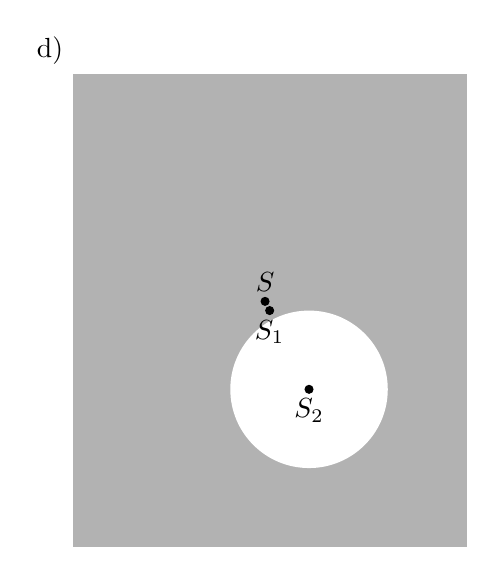
\begin{tikzpicture}
	\draw (0,0) node [above left] {d)};
	\fill [color=black!30] (0,0) rectangle (5,-6);
	\fill [color=white] (3,-4) circle (1cm);
	
	%Teilschwerpunkt S1
	\coordinate (S1) at (2.5,-3);
	\draw [fill] (S1) circle (0.05) node [below] {$S_1$};
	%Teilschwerpunkt S2
	\coordinate (S2) at (3,-4);
	\draw [fill] (S2) circle (0.05) node [below] {$S_2$};

	%Schwerpunkt liegt bei
	\coordinate (S) at (2.4415,-2.8830);
	\draw [fill] (S) circle (0.05) node [above] {$S$};


\end{tikzpicture}

	Den Urspring des Koordinatensystems lege ich an die ober linke Ecke der Gesamtfläche.

	Mit dem gewählten Ursprung des Koordinatensystems liegt der Teilschwerpunkt $S_1$ (Gesamtfläche ohne Loch) bei der Koordinate $(\num{2.5};\num{-3})$,
	diese Fläche ist \SI{30}{cm^2} gross.
	Der Teilschwerpunkt $S_2$ (Kreisfläche) liegt bei $(\num{3};\num{-4})$, der Radius dieser Fläche ist \SI{1}{cm} gross, damit ist diese Fläche $\SI{\pi}{cm^2}$ gross.

	Der Schwerpunkt der Gesamtfläche liegt bei
	\begin{eqnarray*}
		\begin{split}
		r_s &=\frac{r_1\cdot A_1 + r_2\cdot A_2}{A_1 + A_2} =\\
		&=\frac{\vect{2.5\\-3}\cdot\SI{30}{cm^2} + \vect{3\\-4}\cdot (-\SI{3.1415}{cm^2})}{\SI{30}{cm^2}-\SI{3.1415}{cm^2}}=\\
            &=\frac{\vect{75\\90} + \vect{-9.4248\\+12.5664}}{\SI{26.858}{cm^2}} =\\
            &=\frac{\vect{65.575\\-77.434}}{\SI{26.858}{cm^2}} =\\
            &=\vect{2.4415\\-2.8830}
		\end{split}
	\end{eqnarray*}



\end{loesung}










\end{aufgabe}

